\documentclass[aspectratio=169,11pt,t]{beamer}
% ============================================================
%  ksa-cs-v2: ksa-cs-lecture-template.tex 스타일 + 한글, v2 덱(16:9)용.
%    - 짙은 네이비 헤드라인 (섹션 이름 + 프레임마다 점)
%    - 꽉 찬 파란 제목 막대, 둥근 그림자 블록
%    - 한글: Noto Sans CJK KR (fontspec)
%  사용:
%    \documentclass[aspectratio=169,11pt,t]{beamer}
%    \input{<..>/theme/ksa-cs-v2.tex}
%  ksa-theme.tex 의 매크로(\kb \kq, ksablue/ksared 등)도 같은 이름으로 둔다
%  -> v2 덱 본문을 거의 그대로 옮길 수 있다.
% ============================================================

\usepackage{fontspec}
\usepackage{amsmath,amssymb}
\usepackage{tikz}
\usepackage{listings}
\usepackage{graphicx}
\usepackage{booktabs}
\usepackage{varwidth}
% enumitem 은 넣지 않는다 (beamer 글머리표가 사라진다)

\defaultfontfeatures{Ligatures=TeX}
\setmainfont{Noto Sans CJK KR}
\setsansfont{Noto Sans CJK KR}
\setmonofont{Noto Sans Mono CJK KR}[Scale=0.92]
\usefonttheme{professionalfonts}

% ---------- 기본 틀 ----------
\usetheme{default}
\useinnertheme[shadow=true]{rounded}
\setbeamertemplate{navigation symbols}{}
\setbeamersize{text margin left=1em,text margin right=1em}

% ---------- 색 (템플릿 원본 값) ----------
\definecolor{navydark}{HTML}{191959}
\definecolor{navydim}{HTML}{8888B0}
\definecolor{navytitle}{HTML}{262686}
\definecolor{navyblue}{HTML}{3333B2}
\definecolor{blockbodybg}{HTML}{E9E9F3}
\definecolor{examplegreen}{HTML}{006000}
\definecolor{examplebg}{HTML}{E5EFE5}
\definecolor{alertred}{HTML}{BF0000}
\definecolor{alertbg}{HTML}{F9E5E5}
% ksa-theme.tex 와 같은 이름 (본문 호환)
\colorlet{ksablue}{navytitle}
\colorlet{ksabluedk}{navydark}
\definecolor{ksagold}{HTML}{D6CBB1}
\definecolor{ksagolddk}{HTML}{A9976B}
\colorlet{ksared}{alertred}
\definecolor{ksagray}{HTML}{5B5B5B}

\setbeamercolor{structure}{fg=navyblue}
\setbeamercolor{alerted text}{fg=alertred}
\setbeamercolor{frametitle}{bg=navytitle,fg=white}
\setbeamercolor{title}{fg=white,bg=navytitle}
\setbeamercolor{block title}{bg=navytitle,fg=white}
\setbeamercolor{block body}{bg=blockbodybg,fg=black}
\setbeamercolor{block title example}{bg=examplegreen,fg=white}
\setbeamercolor{block body example}{bg=examplebg,fg=black}
\setbeamercolor{block title alerted}{bg=alertred,fg=white}
\setbeamercolor{block body alerted}{bg=alertbg,fg=black}
\setbeamercolor{item}{fg=navyblue}
\setbeamertemplate{itemize item}[circle]
\setbeamertemplate{itemize subitem}[triangle]

% ---------- 헤드라인: miniframes (섹션 이름 + 점) ----------
\useoutertheme[subsection=false]{miniframes}
\setbeamerfont{section in head/foot}{size=\tiny}
\setbeamercolor{section in head/foot}{bg=navydark,fg=white}
\setbeamercolor{mini frame}{fg=white}
\setbeamertemplate{mini frames}[circle]

% ---------- 제목 막대: 폭 꽉 채움, 두 줄까지 ----------
\setbeamerfont{frametitle}{size=\normalsize,series=\bfseries}
\setbeamertemplate{frametitle}{%
  \nointerlineskip
  \begin{beamercolorbox}[wd=\paperwidth,ht=2.7ex,dp=1.1ex,leftskip=.3cm,rightskip=.3cm]{frametitle}%
    \usebeamerfont{frametitle}\insertframetitle
  \end{beamercolorbox}}

% ---------- 쪽 번호: 오른쪽 아래 ----------
\setbeamertemplate{footline}{%
  \hfill
  {\color{navydim}\scriptsize\insertframenumber\,/\,\inserttotalframenumber}%
  \hspace{3mm}\vspace{2mm}%
}

% ---------- 표지: 템플릿처럼 헤드라인은 그대로, 가운데 둥근 그림자 상자에 제목 한 줄 ----------
% 덱에서:  {\setbeamertemplate{footline}{}\begin{frame}[c,noframenumbering]\titlepage\end{frame}}
\setbeamercolor{title}{fg=white,bg=navyblue}
\makeatletter
\setbeamertemplate{title page}{%
  \vfill
  \centering
  \begin{minipage}{0.84\paperwidth}
  \begin{beamercolorbox}[wd=\linewidth,sep=7pt,center,rounded=true,shadow=true]{title}
    {\usebeamerfont{title}\inserttitle\par}%
    \ifx\insertsubtitle\@empty\else\vskip0.4em{\usebeamerfont{subtitle}\insertsubtitle\par}\fi
  \end{beamercolorbox}
  \end{minipage}\par\vskip1.6em
  {\usebeamerfont{author}\color{navytitle}\insertauthor\par}\vskip0.3em
  {\usebeamerfont{institute}\color{ksagray}\insertinstitute\par}
  \vfill
}
\makeatother
\setbeamerfont{title}{series=\bfseries,size=\Large}
\setbeamerfont{subtitle}{size=\normalsize}
\setbeamerfont{author}{size=\normalsize}
\setbeamerfont{institute}{size=\small}

% ksa-theme 호환: 덱이 \renewcommand{\ksacredit}{..} 를 해도 되게 (꼬리말에는 안 쓴다)
\newcommand{\ksacredit}{}

% ---------- 강조 ----------
\newcommand{\hl}[1]{\textcolor{alertred}{#1}}
\newcommand{\hlb}[1]{\textcolor{navyblue}{#1}}
\newcommand{\kb}[1]{\textbf{\color{ksablue}#1}}
\newcommand{\kq}[1]{\textbf{\color{ksared}#1}}

% ---------- 파이썬 코드 (템플릿과 같은 색) ----------
\definecolor{codekw}{HTML}{0033B3}
\definecolor{codebuiltin}{HTML}{BF0000}
\definecolor{codestr}{HTML}{067D17}
\definecolor{codecomment}{HTML}{8C8C8C}
\definecolor{codenum}{HTML}{1750EB}
\lstdefinestyle{py}{
  language=Python, basicstyle=\ttfamily\scriptsize,
  keywordstyle=\color{codekw}\bfseries, stringstyle=\color{codestr},
  commentstyle=\color{codecomment}\itshape, numberstyle=\color{codenum},
  emph={print,len,range,sum,input,int,str,float,list,dict,append,remove,sorted,abs,min,max},
  emphstyle=\color{codebuiltin}, showstringspaces=false, keepspaces=true,
  columns=fixed, basewidth=0.52em, aboveskip=1mm, belowskip=1mm, xleftmargin=2mm,
  breaklines=true
}
\lstset{style=py}

% 원본 덱 (ksa-theme): slides/v2/ml1/week15/vae/ -- 그림은 거기 figs/ 를 그대로 쓴다
\setbeamerfont{author}{size=\normalsize}
\setbeamerfont{institute}{size=\small}
\graphicspath{{../../../v2/ml1/week15/vae/figs/}{../../../assets/}}
\makeatletter
\newcommand{\markpage}[1]{\protected@write\@auxout{}{\string\newlabel{#1}{{\the\c@framenumber}{}}}\hypertarget{#1}{}}
\newcommand{\pref}[1]{\hyperlink{#1}{\textcolor{ksagolddk}{(p.\ref{#1})}}}
\makeatother

\renewcommand{\ksacredit}{Machine Learning and Deep Learning \,\textperiodcentered\, VAE}
\title{VAE 변분 오토인코더 (Variational Autoencoder)}
\subtitle{점 대신 구름으로 줄이면 새 그림을 뽑을 수 있다}
\author{Machine Learning and Deep Learning}
\institute{한국과학영재학교 (KSA)}
\date{}
\begin{document}
{\setbeamertemplate{footline}{}\begin{frame}[c,noframenumbering]\titlepage\end{frame}}


\section{질문}
% --- 오늘의 질문
\begin{frame}{오늘의 질문: 본 적 없는 새 손글씨를 만들려면?}
\vfill
\centering
{\large 지금까지: 그림 $\to$ 이름표 (분류) \quad 오늘: 숫자 몇 개 $\to$ \kb{새 그림} (생성)}\vskip0.8em
\renewcommand{\arraystretch}{1.5}
{\large\begin{tabular}{ll}
오토인코더 (AE) & 그림 $\to$ \textbf{숫자 2개} $\to$ 다시 그림 \quad (인코더 · 디코더)\\
아이디어 & 디코더에 아무 숫자 2개나 넣으면 새 그림?\\
문제 & ``아무 숫자'' 를 어디서 뽑지?
\end{tabular}}\vskip0.6em
{\small 데이터: 손글씨 숫자 1,797장 (8 × 8), 잠재 공간 2칸 (지도처럼 그릴 수 있게)}
\vfill
\note{지금까지는 그림을 보고 이름표를 붙이는 분류를 주로 했습니다. 오늘은 반대로 숫자 몇 개에서 새 그림을 만드는 생성을 배웁니다. 출발점은 오토인코더입니다. 인코더가 그림을 숫자 2개로 줄이고, 디코더가 그 숫자 2개에서 다시 그림을 되살리도록 학습합니다. 그러면 디코더에 아무 숫자 2개나 넣으면 새 그림이 나오지 않을까요? 문제는 그 아무 숫자를 어디서 뽑느냐입니다. 손글씨 숫자 1797장으로, 지도처럼 그릴 수 있게 2칸으로 줄여 실험해 봤습니다.}
\end{frame}

\section{구름}
% --- AE 의 지도
\begin{frame}{오토인코더의 지도: 어디서 뽑아야 할지 모른다}
\markpage{maps}
\vfill
\centering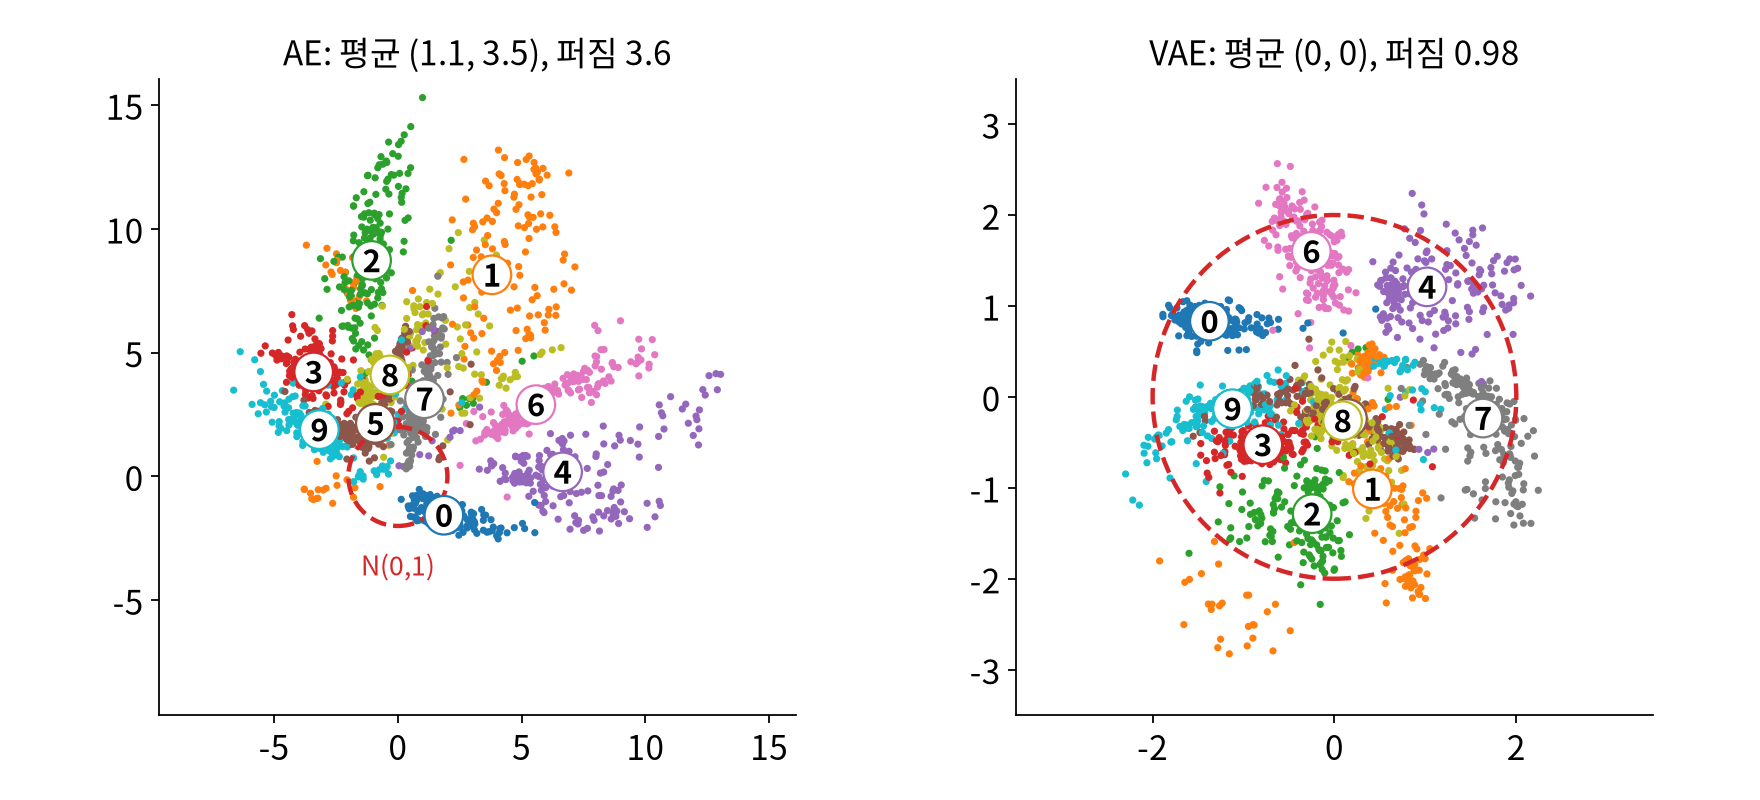
\includegraphics[width=0.78\linewidth]{vae_maps.png}\par\vskip0.1em
{\large AE: 숫자들이 평균 (1.1, 3.5), 퍼짐 3.6 근처에 \textbf{제멋대로} \quad VAE: 평균 0, 퍼짐 \kb{0.98}}\\[0.2em]
{\small 빨간 점선 = 표준정규분포 N(0, 1) 의 95\% 가 들어가는 원 (반지름 2)}
\vfill
\note{같은 구조로 오토인코더와 오늘 배울 VAE를 학습해 2칸 지도를 그렸습니다. 오토인코더의 지도는 숫자들이 평균 1.1, 3.5, 퍼짐 3.6 근처에 제멋대로 퍼져 있습니다. 이 범위는 학습할 때마다 달라지니, 새 그림을 만들려 해도 어디서 숫자를 뽑아야 할지 모릅니다. VAE의 지도는 평균 0, 퍼짐 0.98, 표준정규분포 N 0 1과 거의 같은 모양입니다. 빨간 점선은 N 0 1의 95퍼센트가 들어가는 원입니다. 그러니 N 0 1에서 뽑으면 됩니다.}
\end{frame}

% --- 점 대신 구름
\begin{frame}{VAE: 점 대신 구름으로 줄인다}
\vfill
\centering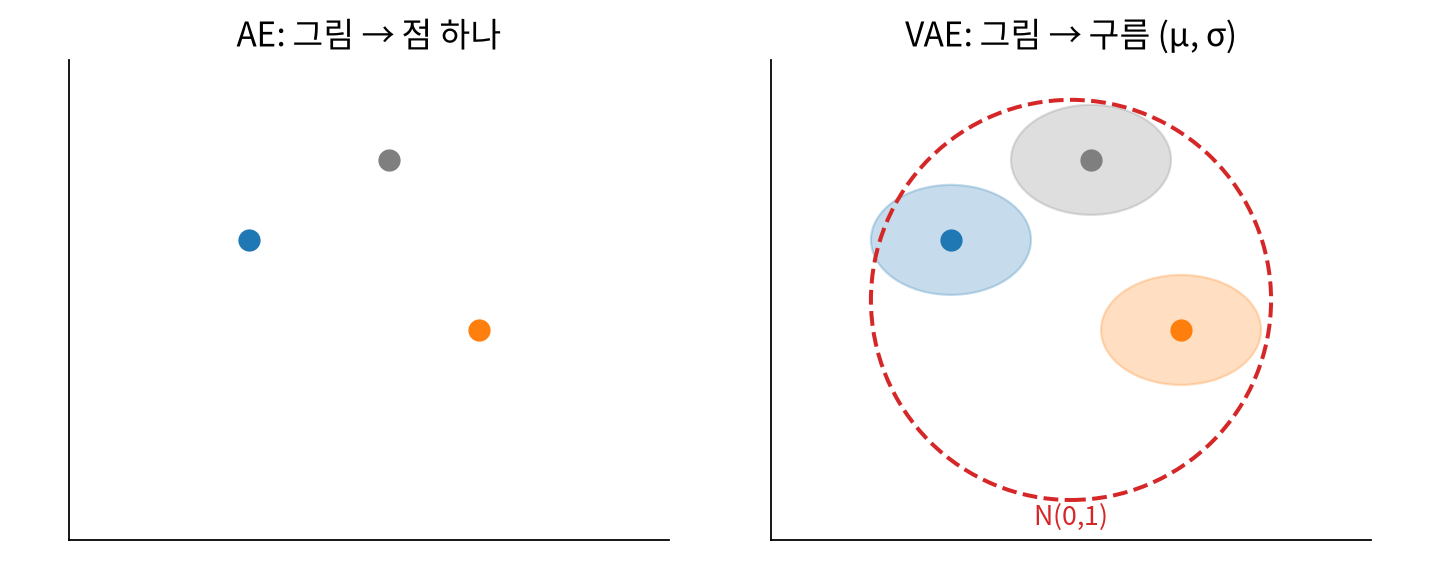
\includegraphics[width=0.63\linewidth]{vae_cloud.png}\par\vskip0.2em
\renewcommand{\arraystretch}{1.4}
{\large\begin{tabular}{ll}
인코더 & 그림 $\to$ 평균 $\boldsymbol{\mu}$ 와 퍼짐 $\boldsymbol{\sigma}$ (구름)\\
뽑기 & 구름에서 한 점 $\mathbf{z} = \boldsymbol{\mu} + \boldsymbol{\sigma} \odot \boldsymbol{\epsilon}$, \quad $\boldsymbol{\epsilon} \sim N(0, 1)$\\
디코더 & $\mathbf{z}$ $\to$ 그림 (구름 \textbf{어디서} 뽑아도 같은 그림이 되도록)
\end{tabular}}\\[0.3em]
{\small Kingma \& Welling (2013) ``Auto-Encoding Variational Bayes''}
\vfill
\note{VAE, 변분 오토인코더는 2013년 킹마와 웰링이 발표했습니다. 핵심은 그림을 점 하나가 아니라 구름으로 줄이는 겁니다. 인코더는 평균 뮤와 퍼짐 시그마를 내고, 그 구름에서 한 점 z를 뽑아 디코더에 넣습니다. 구름 어디서 뽑아도 같은 그림이 되살아나야 하니, 구름 사이 빈틈도 그럴듯한 그림으로 채워집니다. z를 뮤 더하기 시그마 곱하기 엡실론으로 뽑는 것을 재매개변수화라 하는데, 무작위성이 엡실론에만 있으니 뮤와 시그마로 기울기가 흘러갈 수 있습니다.}
\end{frame}

% --- 손실
\begin{frame}{손실 = 복원 + KL}
\markpage{loss}
\vfill
\centering
{\LARGE\[ \text{손실} = \underbrace{\text{복원 오차}(\mathbf{x}, \hat{\mathbf{x}})}_{\text{되살리기}} + \underbrace{\text{KL}\big(N(\boldsymbol{\mu}, \boldsymbol{\sigma}^2) \,\|\, N(0, 1)\big)}_{\text{구름을 N(0,1) 쪽으로}} \]}\vskip0.4em
{\large 칸 하나의 KL \quad $= \dfrac{1}{2}\left(\mu^2 + \sigma^2 - 1 - \ln \sigma^2\right)$}\\[0.6em]
{\large $\mu = 1$, $\sigma = 0.5$: \ $\frac12 (1 + 0.25 - 1 - \ln 0.25) = \frac12 (0.25 + 1.386) = \kb{0.82}$}\\[0.3em]
{\large $\mu = 0$, $\sigma = 1$ 이면 0 \quad 원점에서 멀거나 너무 작거나 크면 벌점}
\vfill
\note{VAE의 손실은 두 항입니다. 첫째는 오토인코더처럼 원래 그림과 되살린 그림의 차이, 복원 오차입니다. 둘째는 구름과 표준정규분포 사이의 KL 발산입니다. KL은 다음 덱에서 자세히 배우는데, 두 분포가 얼마나 다른지 재는 값입니다. 칸 하나에 대해 2분의 1 곱하기 뮤 제곱 더하기 시그마 제곱 빼기 1 빼기 로그 시그마 제곱입니다. 뮤가 1, 시그마가 0.5면 0.82입니다. 뮤가 0, 시그마가 1이면 0이 됩니다. 구름이 원점에서 멀거나, 점처럼 너무 작아지면 벌점을 받습니다. 그래서 VAE의 지도는 N 0 1 모양이 됩니다.}
\end{frame}

% --- 손 계산: 뽑기
\begin{frame}{손으로 한 번: 구름에서 뽑기}
\vfill
\centering
{\large 인코더가 낸 구름: $\mu = 1$, $\sigma = 0.5$ \quad 이번에 뽑은 $\epsilon = -0.4$}\vskip0.6em
{\LARGE\[ z = \mu + \sigma \epsilon = 1 + 0.5 \times (-0.4) = \kb{0.8} \]}\vskip0.4em
{\large 다음 바퀴엔 다른 $\epsilon$ $\to$ 디코더는 0.8 \textbf{근처 어디서든} 같은 그림을}\\[0.6em]
{\large $\dfrac{\partial z}{\partial \mu} = 1, \quad \dfrac{\partial z}{\partial \sigma} = \epsilon = -0.4$ \quad 무작위인데도 기울기가 흐른다}
\vfill
\note{구름에서 뽑는 걸 직접 해 봅시다. 인코더가 뮤 1, 시그마 0.5를 냈고, 이번에 표준정규분포에서 엡실론 마이너스 0.4를 뽑았습니다. z는 1 더하기 0.5 곱하기 마이너스 0.4, 0.8입니다. 다음 바퀴에는 다른 엡실론이 뽑혀 z가 달라지니, 디코더는 0.8 근처 어디서든 같은 그림을 내도록 배웁니다. 그리고 z를 뮤로 미분하면 1, 시그마로 미분하면 엡실론이니, 무작위로 뽑았는데도 기울기가 뮤와 시그마로 흐릅니다.}
\end{frame}

\section{실험}
% --- 실험: 뽑기
\begin{frame}{실험: N(0, 1) 에서 뽑아 되살리기}
\markpage{samples}
\vfill
\centering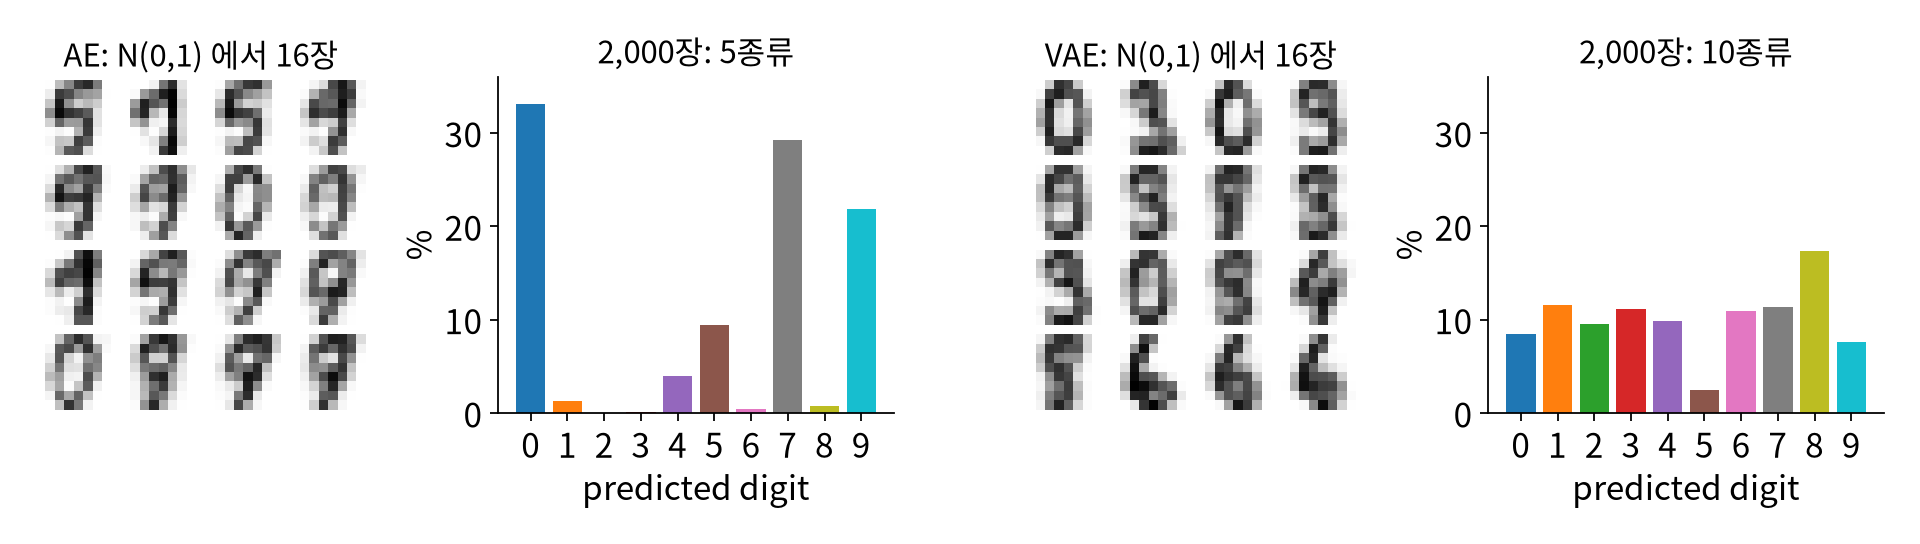
\includegraphics[width=0.92\linewidth]{vae_samples.png}\par\vskip0.2em
{\large AE: 0 · 7 · 9 에 몰리고 \kq{5}종류 \quad VAE: \kb{10}종류 모두 (2 $\sim$ 17\%)}\\[0.2em]
{\small 숫자 판정 = 원본 그림으로 학습한 로지스틱 회귀 \quad 2\% 이상 나온 숫자만 셈}
\vfill
\note{N 0 1에서 숫자 2개를 2000번 뽑아 디코더로 되살렸습니다. 어떤 숫자인지는 원본 그림으로 학습한 분류기로 판정했습니다. 오토인코더는 0, 7, 9에 몰려 다섯 종류만 나왔습니다. N 0 1의 원이 오토인코더 지도의 한 귀퉁이만 덮기 때문입니다. VAE는 열 종류가 모두 2에서 17퍼센트씩 고르게 나옵니다. 지도 전체가 N 0 1 원 안에 들어 있으니까요.}
\end{frame}

% --- 지도 전체
\begin{frame}{VAE 지도 어디를 찍어도 숫자}
\vfill
\begin{columns}[c]
\column{0.45\linewidth}\centering
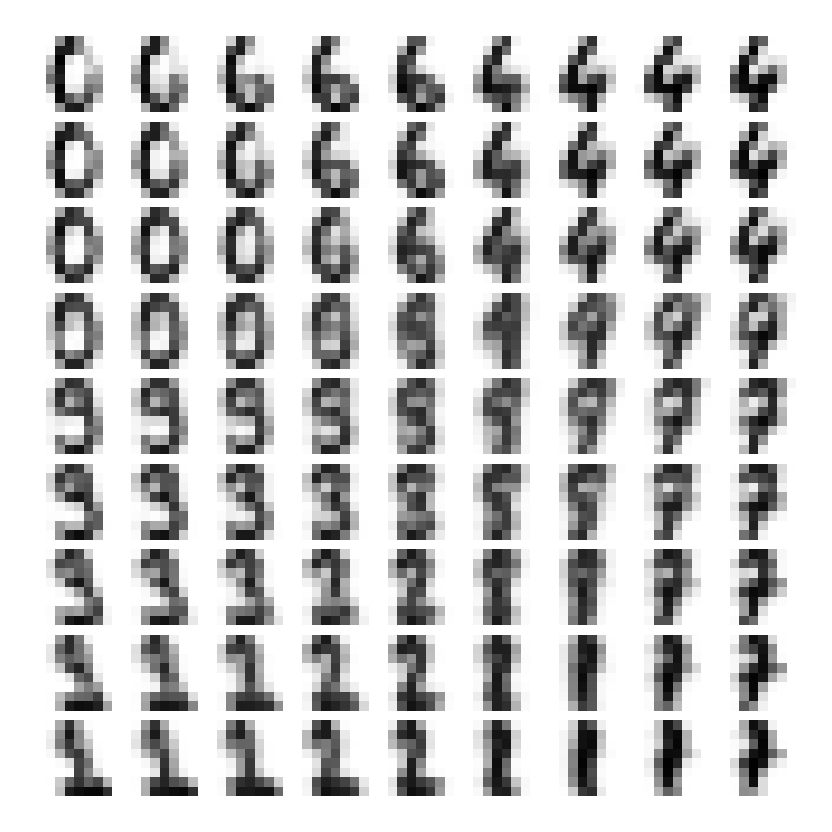
\includegraphics[width=0.80\linewidth]{vae_grid.png}\\
{\small 지도의 $-2 \sim 2$ 를 9 × 9 로 되살림}
\column{0.53\linewidth}
{\large 빈틈 없이 이어진다: 옆 칸은 비슷한 그림}\\[0.8em]
{\large 숫자 0 의 평균 $\to$ 숫자 1 의 평균으로 걷기:}\\[0.3em]

\includegraphics[width=\linewidth]{vae_walk.png}\\[0.6em]
{\large 대가: 복원은 조금 흐리다 \quad 오차 AE 1.85 vs VAE \kq{2.10}}
\end{columns}
\vfill
\note{VAE 지도의 마이너스 2부터 2까지를 9 곱하기 9로 나눠 모두 되살렸습니다. 어디를 찍어도 숫자 모양이 나오고, 옆 칸끼리는 비슷한 그림입니다. 숫자 0들의 평균 위치에서 숫자 1들의 평균 위치로 걸어가면 0이 서서히 1로 바뀝니다. 대가도 있습니다. 구름 어디서 뽑아도 같은 그림을 내야 하니 복원이 조금 흐립니다. 복원 오차는 오토인코더 1.85, VAE 2.10이었습니다.}
\end{frame}

\section{쓰임}
% --- 쓰임
\begin{frame}{어디에 쓰나}
\vfill
\centering
\renewcommand{\arraystretch}{1.5}
{\large\begin{tabular}{ll}
그림 압축 & Stable Diffusion: 512 × 512 그림 $\to$ 64 × 64 × 4\\
분자 설계 & 잠재 공간에서 좋은 성질 쪽으로 걸어가며 새 분자 (2018)\\
이상 탐지 & 잘 되살리지 못하는 데이터 = 평소와 다른 것\\
표현 학습 & 이름표 없이 데이터의 요약 벡터
\end{tabular}}\vskip0.8em
{\large 약점: 그림이 흐리다 $\to$ 선명한 생성은 GAN (2014) · 확산 모델 (2020)}
\vfill
\note{VAE 계열은 그림 압축에 많이 쓰입니다. Stable Diffusion은 512 곱하기 512 그림을 64 곱하기 64 곱하기 4로 줄이는 오토인코더를 쓰는데, VAE와 비슷하게 KL 벌점을 줍니다. 2018년에는 분자를 잠재 공간에 넣고 좋은 성질 쪽으로 걸어가며 새 분자를 설계하는 연구도 나왔습니다. 잘 되살리지 못하는 데이터를 이상한 데이터로 보는 이상 탐지에도 쓰입니다. 약점은 그림이 흐리다는 건데, 선명한 생성은 다음 덱의 GAN과 확산 모델이 맡습니다.}
\end{frame}

\section{연습}
% --- 문제풀이
\begin{frame}{문제풀이}
\vfill
\begin{enumerate}
\item $\mu = 0$, $\sigma = 2$ 인 칸의 KL 은? ($\ln 4 \approx 1.386$) \quad $\mu = 2$, $\sigma = 1$ 이면?\vskip0.8em
\item $\mu = (1, -1)$, $\sigma = (0.5, 2)$, $\epsilon = (2, 0.5)$ 이면 $\mathbf{z}$ 는?\vskip0.8em
\item KL 항을 빼고 학습하면 VAE 는 무엇과 같아질까? 지도는 어떻게 될까?\vskip0.8em
\item KL 항에 큰 가중치 (예: 100배) 를 주면 복원은 어떻게 될까?
\end{enumerate}
\vfill
\note{1번 답. 뮤 0, 시그마 2면 2분의 1 곱하기 0 더하기 4 빼기 1 빼기 1.386, 약 0.81입니다. 뮤 2, 시그마 1이면 2분의 1 곱하기 4, 2입니다. 2번 답. 1 더하기 0.5 곱하기 2는 2, 마이너스 1 더하기 2 곱하기 0.5는 0, z는 2, 0입니다. 3번 답. 구름을 점으로 줄여도 벌점이 없으니 시그마가 0으로 가서 오토인코더와 같아지고, 지도도 제멋대로 퍼집니다. 4번 답. 모든 구름이 N 0 1에 겹쳐 그림 정보를 담지 못하니, 복원이 모두 비슷한 흐린 평균 그림이 됩니다.}
\end{frame}

% --- 실습
\begin{frame}{실습}
\vfill
\centering\begin{tabular}{rl}
\large 1 & KL 손 계산 · 재매개변수화 $z = \mu + \sigma \epsilon$\\[0.5em]
\large 2 & 손글씨 숫자로 AE 와 VAE 학습 (PyTorch) $\to$ 2칸 지도 비교\\[0.5em]
\large 3 & N(0, 1) 에서 뽑아 되살리기 · 지도 격자 · 0 $\to$ 1 걷기
\end{tabular}\vskip1em
\href{https://colab.research.google.com/github/SuminHan/book-ml/blob/main/slides/v2/ml1/week15/vae/lab/vae.ipynb}{\textcolor{ksagolddk}{▶ Colab에서 실습 노트북 열기}}
\vfill
\note{실습은 세 부분입니다. 첫째, KL을 손으로 계산하고 재매개변수화를 확인합니다. 둘째, 손글씨 숫자로 오토인코더와 VAE를 학습해 2칸 지도를 비교합니다. 셋째, N 0 1에서 뽑아 되살리고, 지도 격자를 그리고, 0에서 1로 걸어 봅니다.}
\end{frame}

\section{정리}
% --- 정리
\begin{frame}{정리}
\vfill
\centering\large\begin{tabular}{l}
\textbf{VAE}: 그림 $\to$ 구름 $(\mu, \sigma)$ $\to$ 뽑은 점 $z = \mu + \sigma\epsilon$ $\to$ 그림 (2013)\\[0.5em]
손실 = 복원 + KL$(N(\mu, \sigma^2) \| N(0, 1))$ \quad $\mu = 1, \sigma = 0.5$ 이면 KL 0.82\\[0.5em]
AE 지도: 평균 (1.1, 3.5) 제멋대로 $\to$ VAE 지도: 평균 0 · 퍼짐 0.98\\[0.5em]
N(0, 1) 에서 뽑으면 AE 5종류 · VAE \kb{10종류} \quad 대가: 조금 흐리다
\end{tabular}
\vfill
\note{정리합니다. VAE는 그림을 평균과 퍼짐을 가진 구름으로 줄이고, 구름에서 뽑은 점으로 그림을 되살립니다. 손실은 복원 오차와, 구름을 N 0 1 쪽으로 당기는 KL입니다. 그 결과 오토인코더의 지도는 제멋대로였지만 VAE의 지도는 평균 0, 퍼짐 1에 가까워져, N 0 1에서 뽑으면 열 종류 숫자가 모두 나왔습니다. 대가는 조금 흐린 그림입니다.}
\end{frame}
\end{document}
